\section{Results}\label{sec:results}
All numbers below are generated by the released analysis script from saved raw results.

\subsection{E1: Software tests}
\begin{table}[t]
\centering
\caption{Automated test suite (pytest, offline fake providers).}
\label{tab:tests}
\footnotesize
\setlength{\tabcolsep}{3.5pt}
\begin{tabular}{lr}
\toprule
Item & Value \\
\midrule
Test cases (files) & 80 (14) \\
Passed / failed / errors & 80 / 0 / 0 \\
Line coverage (app) & 65.9\% of 3644 statements \\
Coverage: core / graphs / services & 93.8 / 66.8 / 54.1\% \\
Coverage: providers / api & 62.7 / 59.5\% \\
Wall time & 41.9 s \\
\bottomrule
\end{tabular}
\end{table}

The suite (Table~\ref{tab:tests}) passes completely; it includes ten regression tests added
for the fixes described in Section~\ref{sec:discussion} (circuit breaker, model selection,
response shape, degraded-output flag, credential check and speech-to-text fallback chain).
Coverage is lowest for the speech-to-text providers and the job runner's media path, which
the offline suite deliberately does not call; those paths are exercised by the live
experiments below.

\subsection{E2: Speech recognition}
\begin{table*}[t]
\centering
\caption{Speech recognition on TED-LIUM~3 talks (WER/CER in \%, Whisper normaliser). The first row is the production configuration inside the live pipeline; the others are cached-stage runs of the same \texttt{transcribe\_file} function, four configurations processed concurrently.}
\label{tab:asr}
\footnotesize
\setlength{\tabcolsep}{3.5pt}
\begin{tabular}{lrrrrrrrrr}
\toprule
Model & Chunk (s) & Talks & Corpus WER & Median & Max & CER & S/D/I & RTF & STT (s) \\
\midrule
3.1-flash-lite (pipeline) & 300 & 18 & 2.19 & 2.22 & 5.45 & 1.15 & 464/224/284 & 0.048 & 43.2 \\
3.1-flash-lite & 120 & 18 & 2.19 & 2.17 & 5.03 & 1.17 & 460/229/279 & 0.037 & 25.5 \\
3.1-flash-lite & 600 & 18 & 2.23 & 2.34 & 5.38 & 1.17 & 463/227/297 & 0.030 & 24.1 \\
3.6-flash & 300 & 18 & 2.10 & 1.89 & 5.10 & 1.09 & 413/242/276 & 0.041 & 30.8 \\
3.7-flash & 300 & 18 & 1.98 & 1.87 & 4.54 & 1.06 & 380/210/285 & 0.106 & 90.7 \\
\bottomrule
\end{tabular}
\end{table*}

\begin{figure}[t]
  \centering
  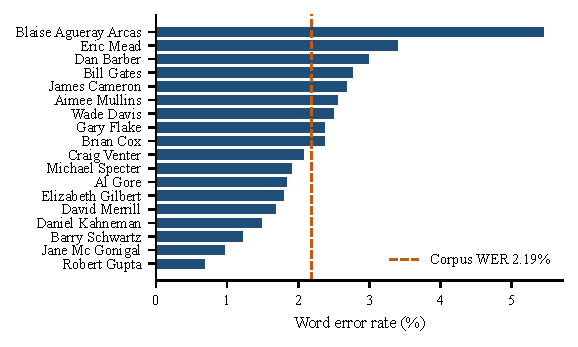
\includegraphics[width=\columnwidth]{fig_wer_per_talk}
  \caption{Per-talk WER of the production configuration (live pipeline, 18 talks).}
  \label{fig:wer}
\end{figure}
In the live pipeline, \texttt{gemini-3.1-flash-lite} with 300\,s quiet-point chunks reaches a
corpus WER of 2.19\% over 44{,}283 reference words (Table~\ref{tab:asr}); per-talk WER ranges
from 0.68\% to 5.45\% (Fig.~\ref{fig:wer}) and the median real-time factor is 0.048; the
longest (25-minute) talk was transcribed in 54\,s. Chunk length barely affects accuracy
(2.19\%, 2.19\% and 2.23\% for 120, 300 and 600\,s windows), which indicates that the
quiet-point splitting does not cut words. The larger \texttt{gemini-3.6-flash} lowers corpus WER
only slightly, to 2.10\%. The newest \texttt{gemini-3.7-flash} is the most accurate (1.98\%)
but more than twice as slow (median RTF 0.106, 90.7\,s per talk), and 10 of its 28
transcription attempts failed---in three talks chunks exceeded the 240\,s per-chunk timeout, the
others coincided with network outages---and were repeated until all 18 talks succeeded. The production choice of \texttt{flash-lite} therefore
trades 0.2 WER points for less than half the transcription time (Fig.~\ref{fig:asrmodels}).
\begin{figure}[t]
  \centering
  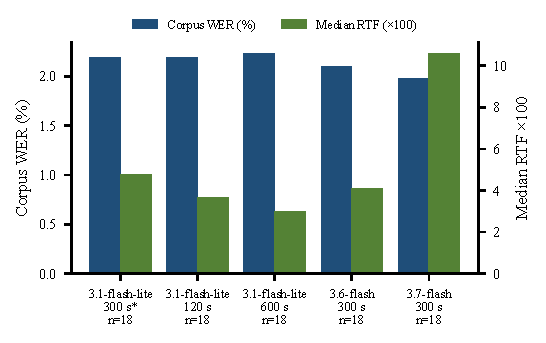
\includegraphics[width=\columnwidth]{fig_asr_models}
  \caption{Corpus WER and median real-time factor by model and chunk length (* = live pipeline).}
  \label{fig:asrmodels}
\end{figure}
Across talks, WER is not related to the judged quality of the drafts (Spearman $\rho=-0.09$,
$n=18$), consistent with the low error rate. Substitutions are the most
frequent error type (464, against 224 deletions and 284 insertions). Transcription consumed 1{,}500--2{,}000 input tokens
per minute of audio, depending on the chunk length.

\subsection{E3: Latency and token usage}
\begin{table}[t]
\centering
\caption{Per-stage latency of the live end-to-end runs (seconds; completed jobs, upload to finished drafts incl.\ Hindi translation).}
\label{tab:latency}
\footnotesize
\setlength{\tabcolsep}{3.5pt}
\begin{tabular}{lrrrr}
\toprule
Stage & $n$ & Median & IQR & Range \\
\midrule
Media check & 18 & 12.30 & 4.55--14.72 & 3.00--155.35 \\
Speech-to-text & 18 & 43.24 & 21.13--51.99 & 8.45--135.53 \\
RAG indexing & 18 & 1.74 & 1.09--2.99 & 0.60--10.09 \\
Analysis & 18 & 3.14 & 2.92--3.27 & 2.64--3.70 \\
RAG retrieval & 18 & 0.57 & 0.00--0.73 & 0.00--0.99 \\
Generation (6 agents) & 18 & 5.41 & 5.02--5.78 & 4.25--10.13 \\
Guardrail (+retry) & 18 & 2.04 & 1.73--2.37 & 1.49--8.40 \\
Translation (hi) & 18 & 12.49 & 11.55--12.92 & 11.10--13.75 \\
\midrule
Total (upload to drafts) & 18 & 90.20 & 56.40--98.20 & 32.90--226.30 \\
\bottomrule
\end{tabular}
\end{table}

\begin{figure}[t]
  \centering
  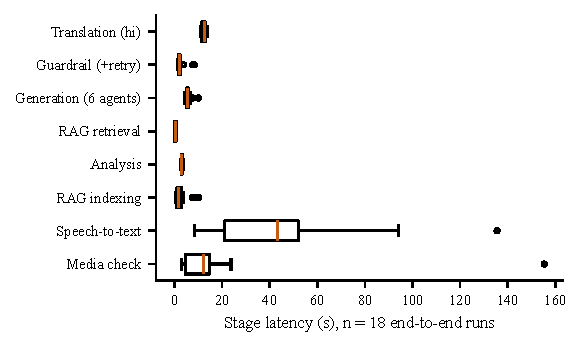
\includegraphics[width=\columnwidth]{fig_latency_stages}
  \caption{Stage latency distribution of the live end-to-end runs.}
  \label{fig:latency}
\end{figure}
\begin{figure}[t]
  \centering
  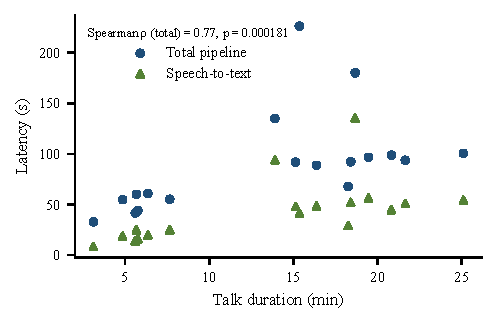
\includegraphics[width=\columnwidth]{fig_latency_vs_duration}
  \caption{Talk duration versus total and speech-to-text latency.}
  \label{fig:latdur}
\end{figure}
A completed job---transcription, analysis, six drafts, guardrail and a Hindi translation of
all drafts---took a median of 90.2\,s (IQR 56.4--98.2\,s) for talks with a median length of
15.2\,min, i.e.\ a median end-to-end real-time factor of 0.12 (Table~\ref{tab:latency},
Fig.~\ref{fig:latency}). Speech-to-text dominates (median 43.2\,s), followed by the local media
check (local silence analysis, median 12.3\,s, with one outlier of 155\,s) and translation
(12.5\,s). Thanks to the parallel fan-out, writing all six drafts takes
only 5.4\,s (median); analysis (3.1\,s), the guardrail (2.0\,s) and RAG retrieval (0.6\,s) are
minor. Total latency grows with talk length (Spearman $\rho=0.77$, $p=1.8\times10^{-4}$,
$n=18$; Fig.~\ref{fig:latdur}). A job made on average 12.8 LLM calls and used 64.5\,k input and
12.0\,k output tokens, of which the six writers account for 28.8\,k input tokens and
transcription for 21.8\,k audio tokens (Fig.~\ref{fig:tokens}).

\begin{figure}[t]
  \centering
  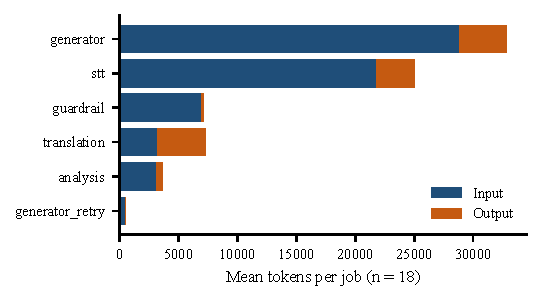
\includegraphics[width=\columnwidth]{fig_tokens_stage}
  \caption{Mean tokens per job by stage (live end-to-end runs).}
  \label{fig:tokens}
\end{figure}

\subsection{E4: Retrieval quality}
\begin{table*}[t]
\centering
\caption{Retrieval on 109 labelled questions over 181 chunks of 11 long talks.}
\label{tab:retrieval}
\footnotesize
\setlength{\tabcolsep}{3.5pt}
\begin{tabular}{llrrrrr}
\toprule
Pool & Retriever & R@1 & R@3 & R@6 & MRR & nDCG@6 \\
\midrule
within-talk & gemini-embedding-001 & 0.76 & 0.98 & 1.00 & 0.87 & 0.90 \\
within-talk & hashed bag-of-words (prev.) & 0.23 & 0.49 & 0.61 & 0.41 & 0.41 \\
within-talk & BM25 & 0.57 & 0.89 & 0.93 & 0.73 & 0.77 \\
\midrule
cross-talk & gemini-embedding-001 & 0.74 & 0.96 & 0.98 & 0.85 & 0.88 \\
cross-talk & hashed bag-of-words (prev.) & 0.06 & 0.14 & 0.21 & 0.13 & 0.12 \\
cross-talk & BM25 & 0.54 & 0.80 & 0.84 & 0.68 & 0.71 \\
\bottomrule
\end{tabular}
\end{table*}

\begin{figure}[t]
  \centering
  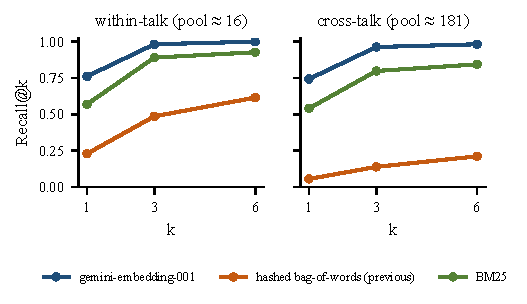
\includegraphics[width=\columnwidth]{fig_retrieval}
  \caption{Recall@$k$ of the three retrievers within a talk and across all talks.}
  \label{fig:retrieval}
\end{figure}
Of 110 generated questions, 109 had a quote found verbatim in the reference and were kept. With
\texttt{gemini-embedding-001}, the relevant chunk is ranked first for 76\% of the questions and
is always within the top six that EventAI passes to the writers (Recall@6 = 1.00, MRR 0.87;
Table~\ref{tab:retrieval}, Fig.~\ref{fig:retrieval}). BM25 is a strong lexical baseline
(MRR 0.73), while the hashed bag-of-words vectors of the previous EventAI version reach only
MRR 0.41. The gap widens in the organisation-memory setting with 181 candidate chunks from
eleven talks: the embedding retriever keeps Recall@6 at 0.98, whereas hashed vectors collapse to
0.21, i.e.\ they could not have supported cross-event memory.

\subsection{E5: Effect of selective RAG}
\begin{table}[t]
\centering
\caption{RAG ablation: same stored transcript, 3 runs per condition, averaged per talk ($n=11$ long talks); two-sided Wilcoxon signed-rank test. Coverage from the automatic judge.}
\label{tab:rag}
\footnotesize
\setlength{\tabcolsep}{2.2pt}
\begin{tabular}{lrrrrr}
\toprule
Metric & RAG off & RAG on & $\Delta$ & $+$/$-$ & $p$ \\
\midrule
Late coverage, all formats (\%) & 46.8 & 68.4 & +21.6 & 10/0 & 0.0020 \\
Early coverage, all formats (\%) & 70.1 & 58.5 & -11.6 & 1/10 & 0.0029 \\
Late coverage, long formats (\%) & 50.8 & 74.7 & +23.9 & 9/0 & 0.0039 \\
All key points, all formats (\%) & 59.8 & 59.1 & -0.7 & 5/5 & 0.7148 \\
\midrule
Factual cons. & 4.96 & 4.99 & +0.03 & 4/1 & 0.1875 \\
Relevance & 5.00 & 4.97 & -0.03 & 0/2 & 0.5000 \\
Completeness & 4.20 & 4.28 & +0.08 & 7/3 & 0.3223 \\
Readability & 5.00 & 4.96 & -0.03 & 1/2 & 0.5000 \\
Instr. adherence & 4.67 & 4.69 & +0.02 & 4/6 & 0.7090 \\
Unsupported claims per draft & 0.04 & 0.01 & -0.04 & 1/5 & 0.1250 \\
\bottomrule
\end{tabular}
\\[2pt]\parbox{\linewidth}{\scriptsize $+$/$-$: talks whose per-talk mean rose/fell with RAG.}
\end{table}

\begin{figure}[t]
  \centering
  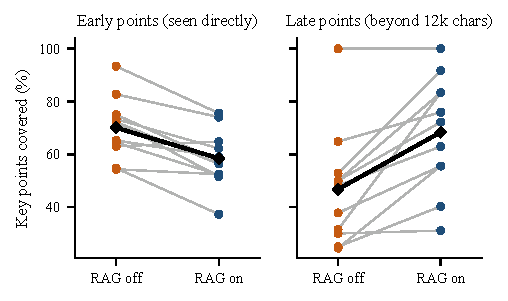
\includegraphics[width=\columnwidth]{fig_rag_ablation}
  \caption{Key-point coverage per talk without and with RAG (grey lines: talks; black: mean).}
  \label{fig:rag}
\end{figure}
On the eleven long talks, RAG raised coverage of key points that lie beyond the writers'
12{,}000-character excerpt from 46.8\% to 68.4\% (+21.6 points; 10 of 11 talks improved, none
worse; $p=0.0020$), and from 50.8\% to 74.7\% for the long formats (Table~\ref{tab:rag},
Fig.~\ref{fig:rag}). Coverage of early points fell from 70.1\% to 58.5\% ($p=0.0029$), and
total coverage was unchanged (59.8\% vs.\ 59.1\%, $p=0.71$): with a fixed output length, RAG
\emph{redistributes} the drafts' attention over the whole talk rather than adding content.
Rubric scores, including factual consistency, did not change significantly, and unsupported
claims stayed rare in both conditions (0.01 vs.\ 0.04 per draft). The \emph{Elizabeth Gilbert}
runs were made after the response-shape fix (Section~\ref{sec:discussion}); without them the
result is the same in direction and significance (late coverage 48.4\% to 72.1\%,
$p=0.0039$, $n=10$). For organisers this means
that, with RAG, posts about long talks no longer ignore their second half.

\subsection{E6: Content quality}
\begin{table*}[t]
\centering
\caption{Automatic-judge quality scores (1--5) of the English drafts of the live end-to-end runs, judged against the human reference transcript.}
\label{tab:quality}
\footnotesize
\setlength{\tabcolsep}{3.5pt}
\begin{tabular}{lrrrrrrr}
\toprule
Format & $n$ & Fact. & Rel. & Compl. & Read. & Instr. & Unsup. \\
\midrule
Summary & 18 & 4.94 & 5.00 & 4.72 & 5.00 & 5.00 & 0.06 \\
Blog & 18 & 5.00 & 5.00 & 4.83 & 5.00 & 4.50 & 0.00 \\
Linkedin & 18 & 5.00 & 5.00 & 4.33 & 5.00 & 4.33 & 0.00 \\
Newsletter & 18 & 4.94 & 5.00 & 4.44 & 5.00 & 4.67 & 0.06 \\
Instagram & 18 & 4.94 & 5.00 & 4.06 & 5.00 & 4.94 & 0.06 \\
Flyer & 18 & 4.94 & 5.00 & 3.72 & 5.00 & 4.44 & 0.06 \\
\midrule
All & 108 & 4.96 & 5.00 & 4.35 & 5.00 & 4.65 & -- \\
\bottomrule
\end{tabular}
\end{table*}

\begin{figure}[t]
  \centering
  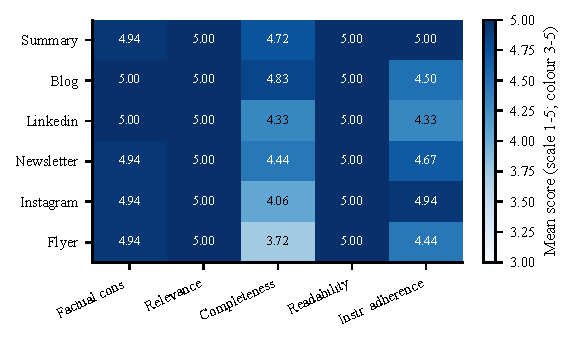
\includegraphics[width=\columnwidth]{fig_quality_heatmap}
  \caption{Mean judge score per format and dimension (colour scale 3--5).}
  \label{fig:quality}
\end{figure}
\begin{table}[t]
\centering
\caption{Deterministic format checks on the end-to-end drafts.}
\label{tab:format}
\footnotesize
\setlength{\tabcolsep}{3.5pt}
\begin{tabular}{lr}
\toprule
Check & Pass \\
\midrule
linkedin 3-5 hashtags & 12/18 \\
linkedin no banned phrases & 18/18 \\
instagram 10-15 hashtags & 18/18 \\
summary <= 400 words & 18/18 \\
flyer no invented date (TBA or none) & 18/18 \\
\bottomrule
\end{tabular}
\end{table}

\begin{table}[t]
\centering
\caption{Agreement between the primary judge (J1, gemini-3.7-flash) and a second judge (J2, gemini-3.6-flash) on the same drafts.}
\label{tab:judge}
\footnotesize
\setlength{\tabcolsep}{3.5pt}
\begin{tabular}{lrrrrrr}
\toprule
Dimension & $n$ & Exact \% & $\pm$1 \% & QWK & J1 & J2 \\
\midrule
Factual cons. & 108 & 90.7 & 100.0 & 0.25 & 4.96 & 4.91 \\
Relevance & 108 & 100.0 & 100.0 & -- & 5.00 & 5.00 \\
Completeness & 108 & 73.1 & 100.0 & 0.62 & 4.35 & 4.32 \\
Readability & 108 & 99.1 & 100.0 & 0.00 & 5.00 & 4.99 \\
Instr. adherence & 108 & 89.8 & 100.0 & 0.88 & 4.65 & 4.69 \\
\bottomrule
\end{tabular}
\end{table}

Judged against the human transcript, the 108 English drafts of the 18 end-to-end
runs score 4.96 for factual consistency with 0--0.06 unsupported claims per draft, 5.00 for
relevance and readability, 4.65 for instruction adherence and 4.35 for completeness
(Table~\ref{tab:quality}, Fig.~\ref{fig:quality}). Completeness is lowest for the short
formats---Instagram (4.06) and especially the flyer (3.72)---which is expected from their
length limits. The deterministic checks (Table~\ref{tab:format}) confirm summary length,
Instagram hashtag counts, absence of banned LinkedIn clich\'es and absence of invented event
dates in all drafts, but only 12 of 18 LinkedIn posts respect the 3--5 hashtag rule. The two
judges agree within one point on every item and exactly on 73.1--100\% of items per dimension
(Table~\ref{tab:judge}); weighted $\kappa$ is 0.62 for completeness and 0.88 for instruction
adherence, and is low or undefined for relevance, readability and factual consistency only
because almost all scores are 5 (the well-known $\kappa$ paradox at a ceiling). The high scores
should therefore be read as ``no defects detected by two LLM judges'' rather than as human
ratings.

\subsection{E7: Reliability}\label{sec:reliability}
\begin{table*}[t]
\centering
\caption{Mock-based fault injection into the production Vertex provider (20 trials per scenario). ``Next call'' is the first model tried by the next call in the same process; ``Flagged'' counts trials whose fallback output was marked as degraded.}
\label{tab:faults}
\footnotesize
\setlength{\tabcolsep}{3.5pt}
\begin{tabular}{llrrlr}
\toprule
Scenario & Outcome (of 20) & Calls & Lat. (s) & Next call & Flagged \\
\midrule
S0 no fault & primary model 20 & 1.0 & 0.00 & 3.1-flash-lite & 0 \\
S1 transient 429 (once) & primary model 20 & 2.0 & 0.00 & 3.1-flash-lite & 0 \\
S2 timeout (once) & primary model 20 & 2.0 & 0.00 & 3.1-flash-lite & 0 \\
S3 persistent 429 on primary & fallback model 20 & 4.0 & 1.01 & 3.1-flash-lite & 0 \\
S4 model 404 not found & fallback model 20 & 2.0 & 0.00 & 3.6-flash & 0 \\
S5 empty response & fallback model 20 & 2.0 & 0.00 & 3.1-flash-lite & 0 \\
S6 JSON in markdown fence & primary model 20 & 1.0 & 0.00 & 3.1-flash-lite & 0 \\
S7 prose, no JSON & unparsed (raw text) 20 & 1.0 & 0.00 & 3.1-flash-lite & 0 \\
S8 all models 500 & offline template 20 & 6.0 & 2.02 & 3.1-flash-lite & 20 \\
\bottomrule
\end{tabular}
\\[2pt]\parbox{\linewidth}{\scriptsize Circuit-breaker probe: 8 consecutive failing calls (fail\_max = 5) reached the upstream 5 times; 3 were short-circuited. Sustained 429 on the primary over 8 calls: the primary was tried by 3 calls, then skipped by its model breaker (fail\_max = 3, 60\,s window).}
\end{table*}

\begin{figure}[t]
  \centering
  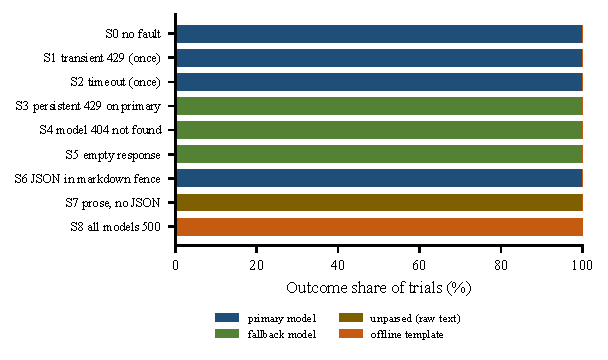
\includegraphics[width=\columnwidth]{fig_fault_injection}
  \caption{Outcomes of mock fault injection (20 trials per scenario).}
  \label{fig:faults}
\end{figure}
\emph{Live.} Across 93 live pipeline runs (84 planned, two repeated after outages and the seven
\emph{Elizabeth Gilbert} runs repeated after the response-shape fix) the backend made 946 model
and embedding calls; 22 failed (2.3\%): 2 rate-limit (429) responses, 7 timeouts and 13 network
errors during host outages. No empty responses and no model fallbacks occurred. The guardrail
triggered a targeted regeneration in 8 runs; after it, 2 of 510 final English drafts (both
newsletters) remained flagged and their jobs were routed to human review. 83 jobs reached
\texttt{pending\_review}, 2 \texttt{needs\_review} and 8 failed: the 7 \emph{Elizabeth Gilbert}
runs before the response-shape fix (all 7 repeated runs after it completed) and 1 from a
network outage combined with an invalid fallback STT credential.

\emph{Mock.} Transient 429s, timeouts, unknown models, empty responses and fenced JSON are all
recovered with usable output (Table~\ref{tab:faults}, Fig.~\ref{fig:faults}); persistent rate
limiting costs about 1\,s before the fallback model answers. Prose without any JSON is still
passed on unparsed. Before the fixes, the next call after an empty response or a persistent
429 stayed on the fallback model (sticky fallback), the circuit breaker short-circuited none of
8 consecutive failing calls, and offline template text was returned without any flag. After
them, the next call returns to the primary model, the breaker rejects 3 of the 8 calls, a
persistently rate-limited primary is skipped from the fourth call on, so later calls no longer
pay the 1\,s, and all 20 trials in which every model failed are flagged as degraded.

\subsection{E8: User-facing workflow}
\begin{figure*}[t]
  \centering
  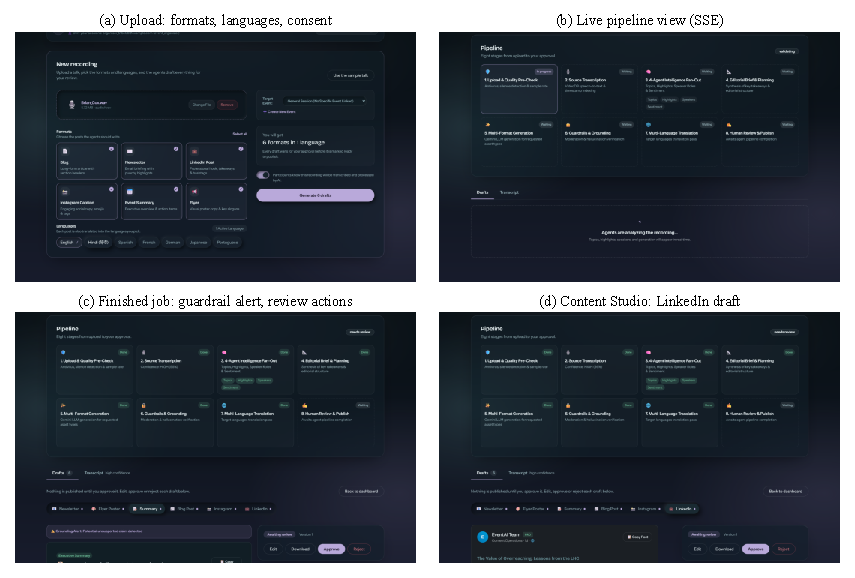
\includegraphics[width=\textwidth]{fig_ui}
  \caption{EventAI web client operated by Playwright on a TED talk: (a) upload with format,
  language and consent selection; (b) live pipeline view; (c) finished job, where the guardrail
  flagged one draft and the job awaits review; (d) a LinkedIn draft in the Content Studio.}
  \label{fig:ui}
\end{figure*}
Fig.~\ref{fig:ui} shows the workflow captured by Playwright on the 3-minute \emph{Brian Cox}
talk: an organiser selects formats, languages and confirms consent, follows the pipeline
stages live and reviews, edits, approves or rejects each draft. In this run the guardrail
flagged the summary and the job correctly stopped at \texttt{needs\_review}. The walkthrough
also exposed a stale label in the client (the transcription stage still named VideoDB, which
the deployment no longer uses); it was corrected after the walkthrough.
